\documentclass[12pt]{article}

%% FONTS
%% To get the default sans serif font in latex, uncomment following line:
 \renewcommand*\familydefault{\sfdefault}
%%
%% to get Arial font as the sans serif font, uncomment following line:
%% \renewcommand{\sfdefault}{phv} % phv is the Arial font
%%
%% to get Helvetica font as the sans serif font, uncomment following line:
% \usepackage{helvet}
\usepackage[small,bf,up]{caption}
\renewcommand{\captionfont}{\footnotesize}
\usepackage[left=1in,right=1in,top=1in,bottom=1in]{geometry}
\usepackage{graphics,epsfig,graphicx,float,subfigure,color}
\usepackage{amsmath,amssymb,amsbsy,amsfonts,amsthm}
\usepackage{url}
\usepackage{boxedminipage}
\usepackage[sf,bf,tiny]{titlesec}
 \usepackage[plainpages=false, colorlinks=true,
   citecolor=blue, filecolor=blue, linkcolor=blue,
   urlcolor=blue]{hyperref}
\usepackage{enumitem}
\usepackage{verbatim}
\usepackage{tikz,pgfplots}
\usepackage{bm}

\newcommand{\todo}[1]{\textcolor{red}{#1}}
% see documentation for titlesec package
% \titleformat{\section}{\large \sffamily \bfseries}
\titlelabel{\thetitle.\,\,\,}

\newcommand{\bs}{\boldsymbol}
\newcommand{\alert}[1]{\textcolor{red}{#1}}
\setlength{\emergencystretch}{20pt}

\begin{document}

\begin{center}
  \vspace*{-2cm}
{\small MATH-GA 2012.004 and CSCI-GA 2945.004, Benjamin Peherstorfer}
\end{center}
\vspace*{.5cm}
\begin{center}
\large \textbf{%%
Spring 2019: Advanced Topics in Numerical Analysis: \\
Stochastic modeling and uncertainty quantification in complex systems \\
Assignment 2 (due Apr.\ 22, 2019) }
\end{center}

\vspace*{0.4cm}
\begin{center}
\large \textbf{Terrence Alsup}
\end{center}

\vspace*{0.25cm}

% The machine used.
%\emph{Note: }

\vspace*{0.25cm}

% ****************************
\begin{enumerate}
% --------------------------

\item {\large \textbf{Smolyak quadrature}}

\hspace{0.5cm} We implement the Smolyak quadrature by creating a sequence of helper functions.  The first is {\tt cheb1D}, which takes in an integer and computes the Clenshaw-Curtis points and weights in 1-dimension.  We use an alternate formula for the points, which is actually the same one that the package Chebfun uses.
\begin{equation}
\label{eq:chebpts}
x_{l,k} = \sin \left( \frac{\pi k }{2(n_l - 1)}  \right) \quad \text{ for } k = -(n-1), -(n-1)+2,\ldots, n-1
\end{equation}
This formula enforces a symmetry so that at the middle point we compute 0 exactly and obtain better accuracy.  Next in our implementation we have a function called {\tt chebdD}, which computes the tensor-product of the Clenshaw-Curtis points for multiple dimensions and calculates the weights by taking the product.  After this we have {\tt incdD} which computes the points and weights for the increments (again tensorized).  Both this function and {\tt chebdD} are recursive in the dimension when computing the tensor-product of the points.  Finally we implement {\tt smolyakdD}, which takes as inputs the level, the dimension, and a function handle.  We use a helper function called {\tt integer\_combinations} that computes all of the possible integer combinations of $d$ variables to achieve a total value.  This is done in a recursive fashion on the dimension again.  Finally, to compute the integral of the function with respect to the quadrature rule we sum over all of the results from the increments.\\


\hspace{0.5cm} We now test our implementation of the Smolyak quadrature on computing the integral
\begin{equation}
\label{eq:integral1}
\int_{[0,1]^d} \left( 1 + 1/d\right)^d \prod_{i=1}^d x_i^{(1/d)} d{\bm x} = 1
\end{equation}
by looking at the relative error as in Table~\ref{table:integral1}.  We see two things.  First is that as we increase the level the relative error of our approximation decreases, indicating that the implementation is working correctly.  The second is that as we increase the dimension the relative error decays much more slowly.  Indeed for $d=6$ we still have a fairly large relative error even at level 10.

\begin{table}[H]
\centering
\begin{tabular}{ | l || r | r | r | r | r | r |}
\hline
Level \textbackslash $d$ & 1 & 2 & 3 & 4 & 5 & 6 \\
\hline
4   & 0.006448 & 0.121020 & 0.357042 & 0.595544 & 0.771527 & 0.880616\\
6   & 0.000402 & 0.022756 & 0.121988 & 0.297871 & 0.497392 & 0.672269\\
8   & 0.000025 & 0.003796 & 0.033994 & 0.119038 & 0.259617 & 0.428249\\
10 & 0.000002 & 0.000593 & 0.008376 & 0.040617 & 0.114351 & 0.231345\\
\hline
\end{tabular}
\caption{The relative error of our Smolyak quadrature rule for the integral~\ref{eq:integral1}.}
\label{table:integral1}
\end{table}

\hspace{0.5cm} We also test our implementation on computing the integral
\begin{equation}
\label{eq:integral2}
\int_{[-1,1]^d} \prod_{i=1}^d \sin\left( \frac{(x_i + 1)\pi}{2}  \right) d{\bm x} = \left(\frac{4}{\pi}\right)^d
\end{equation}
and have recorded the relative error in Table~\ref{table:integral2} below.  We again see that increasing the level greatly improves the accuracy, but increasing the dimension results in slower convergence.  Additionally, we notice that these relative errors are much smaller and converge to zero much faster than when calculating \ref{eq:integral1}.  This agrees with the theory behind sparse grids because the function we are integrating in \ref{eq:integral2} is much smoother.  Thus, we would expect faster convergence.
\begin{table}[H]
\centering
\begin{tabular}{ | l || r | r | r | r | r | r |}
\hline
Level \textbackslash $d$ & 1 & 2 & 3 & 4 & 5 & 6 \\
\hline
1 & 0.047198 & 0.096623 & 0.148381 & 0.202581 & 0.259340 & 0.318778\\
2 & 0.000296 & 0.001607 & 0.005918 & 0.012860 & 0.022672 & 0.035609\\
3 & 0.000000 & 0.000028 & 0.000018 & 0.000252 & 0.000807 & 0.001832\\
4 & 0.000000 & 0.000000 & 0.000002 & 0.000003 & 0.000005 & 0.000037\\
\hline
\end{tabular}
\caption{The relative error of our Smolyak quadrature rule for the integral~\ref{eq:integral1}.}
\label{table:integral2}
\end{table}


\item {\large \textbf{Stochastic collocation}}

\hspace{0.5cm}  We now test our implementation on the model problem with ${\bm \xi} = [\xi_1,\ldots, \xi_d]$ and $\xi_i \sim \text{Uniform}[1,10]$ are i.i.d.  We write $Q(u; {\bm \xi})$ to denote our quantity of interest which depends implicitly on ${\bm \xi}$, and we calculate the expectation by
\begin{equation}
\label{eq:expectation}
\mathbb{E}_{\bm \xi}[Q(u)] = \frac{1}{9^d} \int_{[1,10]^d} Q(u; {\bm \xi})\ d{\bm \xi}.
\end{equation}
To fit with our implementation, which can only integrate over $[-1,1]^d$, we use the change of variables $x_i = \frac{2}{9}\xi_i - \frac{11}{9}$.  Now the integral becomes
\begin{equation}
\label{eq:change_of_variables}
\mathbb{E}_{\bm \xi}[Q(u)] = \frac{1}{2^d} \int_{[-1,1]^d} Q(u; {\bm x})\ d{\bm x}.
\end{equation}
We compare the Smolyak quadrature with the Monte Carlo estimator
\begin{equation}
\label{eq:montecarlo}
\mathbb{E}_{\bm \xi}[Q(u)] \approx \frac{1}{N}\sum_{i=1}^N Q(u^{(i)}; {\bm \xi}^{(i)}), \quad \quad {\bm \xi}^{(i)} \text{ i.i.d. }
\end{equation}


\hspace{0.5cm} For $d=2$ we split the domain evenly into a top half $\{(x_1,x_2) : x_2 \in (0.5,\ 1]\} $ and a bottom half $\{(x_1,x_2) : x_2 \in [0,\ 0.5]\}$ in the function {\tt coeffFun2DBlocks2}.  Since we are in 2 dimensions, we can calculate a reference value $Q_{\text{ref}}$ using Matlab's built-in {\tt integral2} function.  Figure~\ref{fig:comparisond2} below shows the comparison between Smolyak quadrature with the Monte Carlo estimator \ref{eq:montecarlo}.  We see that Smolyak quadrature performs significantly better than Monte Carlo and has an extremely fast rate of decay for the error.  This is a result of our quantity of interest $Q(u, {\bm \xi})$ depending smoothly on the parameter ${\bm \xi}$.  Monte Carlo has no way to take advantage of this and is why we observe the usual rate of $1/2$.


\begin{figure}[H]
\centering
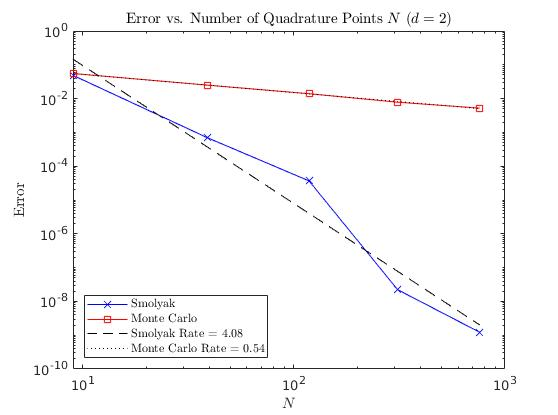
\includegraphics[width=5in]{smolyak_mc_error_d2.jpg}
\caption{The rate of convergence for Smolyak quadrature and Monte Carlo for computing the integral \ref{eq:expectation} when $d=2$. Note that the solution $Q(u)$ itself is approximated with finite elements using level $\ell = 4$.  For Monte Carlo we estimate the root-mean-squared-error (RMSE) using 100 trials.}
\label{fig:comparisond2}
\end{figure}

\hspace{0.5cm} Similarly, we can increase the dimension to $d=6$ by splitting the domain into 6 regions
\begin{equation}
\label{eq:domains}
\Omega_i = \left\{(x_1,x_2)\ :\  \frac{1}{6}(i-1) \le x_2 < \frac{1}{6}i  \right\} \quad i=1,2,\ldots,6,
\end{equation}
which is done with the Matlab function {\tt coeffFun2DBlocks6}.  Since there is no built-in Matlab function to compute this 6-dimensional integral we calculate a reference value $Q_{\text{ref}}$ by using the Smolyak quadrature (now that it has been tested) with sparse grids of level 4 (note this is different from the level $\ell = 2$ used to solve the PDE).  Figure~\ref{fig:comparisond6} below shows the results for sparse grid levels $1,2,3$.  As expected Smolyak quadrature again performs better than Monte Carlo although this time the rate is slower.  This is a result of solving a higher-dimensional integral.  It is also potentially the result of less regularity of $Q(u; {\bm \xi})$.  We note that here we used the level $\ell = 2$ when solving for $Q(u)$ whereas before we had used $\ell = 4$.  This was an attempt to greatly reduce computational cost.


\begin{figure}[H]
\centering
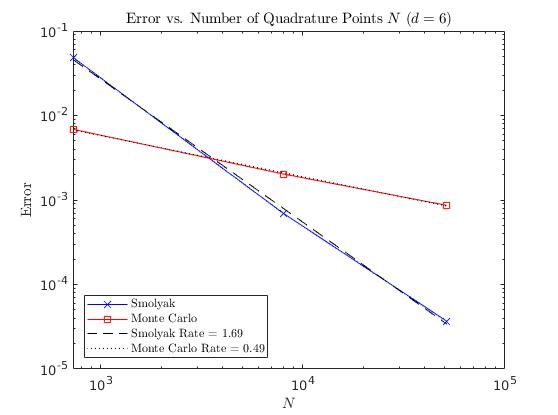
\includegraphics[width=5in]{smolyak_mc_error_d6.jpg}
\caption{The rate of convergence for Smolyak quadrature and Monte Carlo for computing the integral \ref{eq:expectation} when $d=6$. Note that the solution $Q(u)$ itself is approximated with finite elements using level $\ell = 2$.  For Monte Carlo we estimate the root-mean-squared-error (RMSE) using 100 trials.}
\label{fig:comparisond6}
\end{figure}


\hspace{0.5cm}  We note that an attempt to go to higher dimensions, particularly $d=16$, fails even for the sparse grids.  The base level has $3$ quadrature points in each dimension.  For 16 dimensions this is $3^{16}$ total quadrature points, which is over 43 million.  This is way too expensive for either Smolyak or Monte Carlo given that each point requires one solve of our PDE, even with parallelization.  Note that for Monte Carlo we could choose to use fewer samples, but would then get a fairly large RMSE.


\end{enumerate}

\end{document}